\documentclass[journal]{IEEEtran}

\usepackage[utf8]{inputenc}
\usepackage[T1]{fontenc}
\usepackage{amsmath,amssymb}
\usepackage{booktabs}
\usepackage{graphicx}
\usepackage{microtype}
\usepackage{multirow}
\usepackage{array}
\usepackage{tabularx}
\usepackage{xcolor}
\usepackage{url}
\usepackage[hidelinks,hypertexnames=false]{hyperref}
\usepackage{algorithm}
\usepackage{algorithmic}
\usepackage[numbers,square,sort&compress]{natbib}

\newcommand{\agentforge}{\textsc{AgentForge}}
\newcommand{\swebench}{\textsc{SWE-bench}}
\newcommand{\ie}{\textit{i.e.,}\ }
\newcommand{\eg}{\textit{e.g.,}\ }
\newcommand{\tbd}[1]{\textcolor{red!70!black}{\textbf{[TBD after leakage-free rerun: #1]}}}
\newcommand{\res}{\textcolor{red!70!black}{\textbf{TBD}}}
\newcommand{\draftwarning}{%
\begin{center}
\fbox{\parbox{0.94\linewidth}{\small\textbf{Revision status.} This draft has been rewritten to address the reviewers' concerns about evaluation leakage, execution semantics, baseline control, and reproducibility. Numerical claims from the rejected version are intentionally not carried forward. Red placeholders must be replaced only with outputs from a leakage-free rerun using the official SWE-bench harness.}}
\end{center}}

\title{AgentForge: A Role-Structured Multi-Agent Framework for Repository-Level Software Repair with Execution Feedback}

\author{%
Rajesh~Kumar,
\thanks{R. Kumar is with the International Research Center for Complexity Sciences, Hangzhou International Innovation Institute, Beihang University, Hangzhou 311115, China (e-mail: rajakumarlohano@gmail.com).}
Waqar~Ali,
\thanks{W. Ali is with the Department of Computer Science, College of Science, Mathematics and Technology, Wenzhou-Kean University, Wenzhou 325060, China (e-mail: waqar.uestc@yahoo.com).}
Junaid~Ahmed,
\thanks{J. Ahmed is with the Department of Computer Systems Engineering, Sukkur IBA University, Sindh, Pakistan (e-mail: j.bhatti@iba-suk.edu.pk).}
Najma~Imtiaz~Ali,
\thanks{N. I. Ali is with the Faculty of Information and Communication Technology, Universiti Teknikal Malaysia Melaka, Melaka 76100, Malaysia (e-mail: najma@utem.edu.my).}
Shaban~Usman%
\thanks{S. Usman is with the Yibin Park of the University of Electronic Science and Technology of China, Yibin 644000, China (e-mail: shabanusman@yahoo.com).}}

\begin{document}
\maketitle
\draftwarning

\begin{abstract}
Repository-level software repair requires more than generating a plausible patch: an agent must inspect a codebase, localize the defect, modify the repository, execute relevant checks, interpret failures, and revise the patch within a limited budget. We present \agentforge{}, a role-structured multi-agent framework that separates planning, editing, test construction, debugging, and review while maintaining a shared repository state and execution history. The revised design introduces an explicit \emph{post-edit execution invariant}: every state-changing edit must be followed by execution in the same repository environment before another edit is permitted. Agent-generated tests are treated as auxiliary debugging signals rather than ground-truth correctness evidence, and final correctness is measured only by the official \swebench{} evaluation harness. We specify a leakage-free protocol that excludes reference patches and benchmark grading metadata from agent-visible inputs, resets episodic memory for each evaluation instance, and compares agent configurations under matched model, tool, token, cost, and execution budgets. \tbd{Insert the official SWE-bench Lite resolution rate, confidence interval, cost, and controlled-ablation findings.} The framework and evaluation artifacts will be released with a frozen commit and task-level predictions.
\end{abstract}

\begin{IEEEkeywords}
Large language models, multi-agent systems, automated program repair, repository-level software engineering, execution feedback, SWE-bench.
\end{IEEEkeywords}

\section{Introduction}
\label{sec:intro}

Large language models (LLMs) can synthesize code from natural-language specifications, but repository-level software repair remains difficult. A realistic repair task requires the system to interpret an issue report, inspect an unfamiliar repository, identify relevant files, modify existing code, execute tests, diagnose failures, and avoid regressions. Function-level benchmarks such as HumanEval emphasize isolated synthesis, whereas \swebench{} evaluates changes to real repositories under project-specific tests and environments~\cite{chen2021codex,jimenez2024swebench}.

Tool-using software engineering agents address part of this challenge by exposing shell, editor, search, and execution interfaces to an LLM~\cite{yang2024sweagent,wang2024openhands,zhang2024autocoderover}. Multi-agent systems add role specialization, assigning planning, coding, testing, or review to separate agents~\cite{tao2024magis,khanzadeh2025agentmesh,hong2023metagpt,qian2023chatdev}. These directions are complementary: tool access supplies interaction with the repository, while decomposition can make intermediate responsibilities explicit. However, claims about the value of execution or multi-agent structure require carefully controlled evaluation. A system with more calls, more tokens, more tools, and more test attempts cannot be fairly compared with a weaker single-call baseline without controlling those resources.

This paper studies a narrower question: \emph{under matched computational and tool budgets, does a role-structured workflow with enforced post-edit execution improve repository-level repair?} We introduce \agentforge{}, a framework with five roles: Planner, Coder, Tester, Debugger, and Critic. The central design feature is not merely that execution tools are available, but that the orchestrator treats execution as a state-machine constraint. After a Coder or Debugger action changes the repository, the system must execute a validation command and record its outcome before another state-changing action can occur.

The revised evaluation is designed around four validity requirements. First, the agent receives only the issue statement and the base repository checkout; reference patches, reference-derived file paths, benchmark test metadata, and grading labels are excluded. Second, execution occurs in the same instance-specific repository environment used during interaction, while final scoring is performed independently through the official \swebench{} harness. Third, generated tests are auxiliary hypotheses and are not equated with benchmark correctness. Fourth, comparisons are paired and budget controlled.

\textbf{Contributions.} This work makes the following contributions:
\begin{itemize}
    \item A role-structured repository-repair architecture that separates planning, editing, auxiliary test generation, debugging, and review while preserving a single mutable repository state.
    \item An explicit post-edit execution invariant enforced by the orchestrator rather than delegated to a planner-generated sequence.
    \item A contamination-resistant evaluation protocol that excludes gold-patch information, isolates episodic memory, and uses the official \swebench{} evaluation infrastructure.
    \item A controlled experimental design that separates the effects of role decomposition, forced execution, tool access, and additional test-time computation under matched budgets.
    \item \tbd{Summarize only findings supported by the new task-level rerun.}
\end{itemize}

The paper deliberately avoids claiming that execution-enabled agents are new. SWE-agent and OpenHands already support iterative interaction with executable environments~\cite{yang2024sweagent,wang2024openhands}. Our contribution is the orchestration policy, its controlled evaluation, and the separation of auxiliary runtime signals from hidden benchmark correctness.

\begin{figure*}[t]
    \centering
    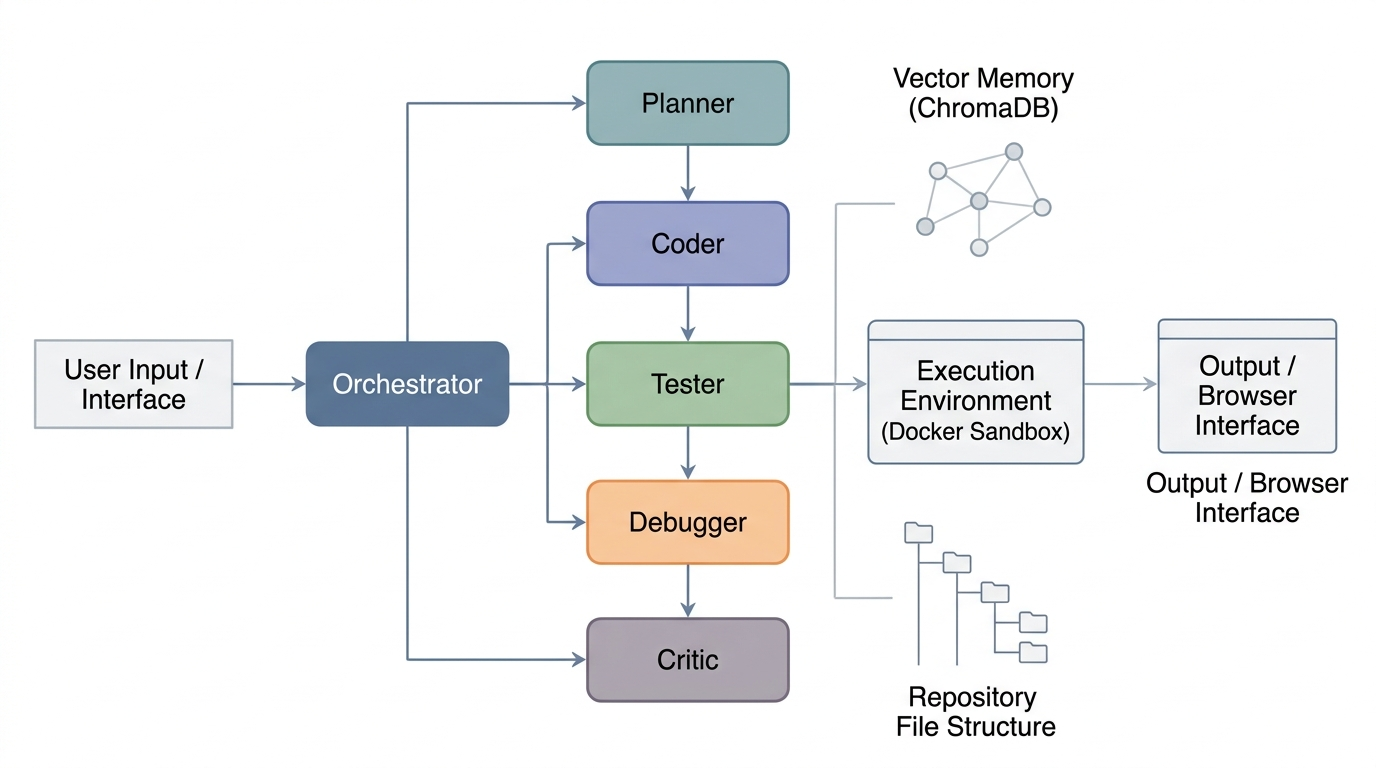
\includegraphics[width=0.92\linewidth]{Figure1.png}
    \caption{Conceptual architecture of \agentforge{}. For benchmark evaluation, the repository is initialized from the base commit, cross-instance memory is disabled, and all state-changing edits are followed by execution in the same task environment. The figure is architectural; the official benchmark harness independently evaluates the final patch.}
    \label{fig:overview}
\end{figure*}

\section{Related Work}
\label{sec:related}

\subsection{Code Generation and Automated Program Repair}

Large pretrained models such as Codex, AlphaCode, StarCoder, and Code Llama established strong code-generation capabilities~\cite{chen2021codex,li2022alphacode,li2023starcoder,roziere2023codellama}. Automated program repair (APR), however, requires a candidate patch to satisfy behavioral constraints in an existing system. Classical APR systems search or synthesize patches using tests and fault-localization signals~\cite{le2012genprog}. More recent LLM-based repair systems use error messages, execution traces, or iterative self-debugging to refine outputs~\cite{xia2022less,jin2023inferfix,fan2023automated,chen2023teaching,olausson2023selfrepair}. These methods motivate the use of runtime evidence, but generated or visible tests can provide incomplete supervision and must not be conflated with hidden benchmark correctness.

\subsection{Tool-Using Software Engineering Agents}

ReAct interleaves reasoning and tool use, and Reflexion adds memory-based self-correction~\cite{yao2023react,shinn2023reflexion}. SWE-agent provides an agent-computer interface for repository navigation, editing, and command execution~\cite{yang2024sweagent}. OpenHands offers an open platform with sandboxed runtime interaction~\cite{wang2024openhands}, while AutoCodeRover combines repository analysis with patch generation~\cite{zhang2024autocoderover}. These systems demonstrate that executable environments are already central to autonomous software engineering. Accordingly, \agentforge{} does not claim novelty for sandbox access itself; it studies an orchestrator-enforced execution schedule under controlled budgets.

\subsection{Multi-Agent Software Engineering}

MetaGPT and ChatDev model software development as communication among specialized roles~\cite{hong2023metagpt,qian2023chatdev}. AutoGen provides a general framework for multi-agent interaction~\cite{wu2023autogen}. MAGIS applies manager, repository-custodian, developer, and QA roles to GitHub issue resolution~\cite{tao2024magis}; AgentMesh similarly explores cooperative role decomposition~\cite{khanzadeh2025agentmesh}. Role specialization can improve modularity and interpretability, but additional agents also increase test-time computation. A convincing evaluation must therefore compare role structures while holding the base model, tool set, context, and resource budget constant.

\subsection{Repository Retrieval and Memory}

Repository-level generation benefits from retrieving relevant files and functions~\cite{zhang2023repocoder,shrivastava2023repofusion}. Retrieval-augmented generation more broadly conditions model outputs on external evidence~\cite{lewis2020rag}. Episodic memory may transfer useful patterns across tasks, as in Reflexion~\cite{shinn2023reflexion}, but evaluation-time memory creates contamination risks when benchmark instances influence later instances. In our primary evaluation, memory is empty and reset for every task. Cross-task memory is treated as a separate experiment and may be populated only from a documented, disjoint training set.

\section{AgentForge}
\label{sec:method}

\subsection{Problem Definition and Information Boundary}

For each task $i$, the agent receives an issue description $q_i$ and a repository checkout $R_i^0$ at the benchmark base commit. The agent produces a patch $p_i$ that transforms the repository into $R_i^*=R_i^0\oplus p_i$. The final patch is successful only if the official benchmark harness accepts it.

The following fields are prohibited from all agent-visible inputs and retrieval indexes during inference:
\begin{itemize}
    \item the reference or gold patch;
    \item file paths extracted from the reference patch;
    \item benchmark grading labels or expected outcomes;
    \item \textsc{fail\_to\_pass} and \textsc{pass\_to\_pass} identifiers;
    \item data derived from other evaluation instances.
\end{itemize}
The agent may inspect only the base repository, the issue statement, command outputs produced during its own run, and optional memory built from a disjoint training set.

\subsection{Roles and Shared State}

\agentforge{} contains five role-specific agents coordinated by a deterministic Orchestrator:

\paragraph{Planner.} The Planner converts the issue description and retrieved repository context into a structured repair plan. The plan may identify investigation steps and candidate validation commands, but it cannot waive the execution invariant.

\paragraph{Coder.} The Coder proposes a minimal patch against the current repository state. Existing files are edited through unified diffs where possible.

\paragraph{Tester.} The Tester may construct auxiliary tests or reproduction scripts from the issue description and inspected code. These artifacts are used for diagnosis only and are labeled as model-generated evidence.

\paragraph{Debugger.} The Debugger receives the current patch, command, exit status, standard output, and standard error. It proposes a revised patch targeted at the observed failure.

\paragraph{Critic.} The Critic reviews the issue, cumulative diff, executed commands, and recorded outcomes. It may stop the search or request another repair iteration, but it cannot declare benchmark success. Only the official harness determines resolution.

All roles operate on one mutable repository state and one append-only execution history. This avoids parallel agents silently reasoning over inconsistent versions of the codebase.

\subsection{Post-Edit Execution Invariant}
\label{sec:invariant}

Let $R_t$ denote the repository state at step $t$. A state-changing action $a_t$ applies a patch and produces $R_{t+1}$. The Orchestrator maintains a Boolean flag $x_t$ indicating whether execution is required. The invariant is
\begin{equation}
  R_{t+1} \neq R_t \;\Rightarrow\; x_{t+1}=1,
\end{equation}
and no subsequent state-changing action is permitted while $x=1$. The flag is cleared only after a command is executed in the same repository environment and its outcome is appended to the history. Thus, execution is enforced by control flow rather than by hoping that the Planner schedules a Tester step.

\begin{algorithm}[t]
\caption{AgentForge repair loop. The execution flag $x$ is owned by the orchestrator, not by the plan; line~\ref{line:guard} is an assertion that fails the run rather than a branch the Planner can influence.}
\label{alg:main}
\begin{algorithmic}[1]
\REQUIRE Issue $q$, base repository $R^0$, budget $B$
\ENSURE Model patch $p$ and trajectory $H$
\STATE $R \leftarrow R^0$; $H \leftarrow [\,]$; $x \leftarrow 0$; memory $\leftarrow \emptyset$
\STATE $C \leftarrow \textsc{Retrieve}(q,R^0)$ \COMMENT{base checkout only}
\STATE $P \leftarrow A_{\mathrm{plan}}(q,C)$; $s \leftarrow A_{\mathrm{test}}(q,C)$
\WHILE{$\textsc{BudgetRemaining}(B)$}
    \STATE \textbf{assert} $x=0$ \COMMENT{no edit while execution is owed}\label{line:guard}
    \STATE $a \leftarrow \mathrm{debugger}$ \textbf{if} $H$ holds a failure \textbf{else} $\mathrm{coder}$
    \STATE $\Delta \leftarrow A_a(q,C,P,H)$
    \STATE $(\mathit{ok},m) \leftarrow \textsc{ApplyPatch}(R,\Delta)$
    \IF{$\neg\,\mathit{ok}$}
        \STATE $H.\textsc{append}(a,\Delta,m)$ \COMMENT{$R$ unchanged, so no execution is owed}
        \STATE \textbf{continue}
    \ENDIF
    \STATE $x \leftarrow 1$ \COMMENT{$R$ changed}
    \STATE $c \leftarrow \textsc{SelectCommand}(q,s)$ \COMMENT{never reads graded test ids}
    \STATE $(z,o,e) \leftarrow \textsc{Execute}(R,c)$
    \STATE $H.\textsc{append}(a,\Delta,c,z,o,e)$; $x \leftarrow 0$
    \IF{$z=0$}
        \STATE $v \leftarrow A_{\mathrm{critic}}(q,\textsc{Diff}(R^0,R),H)$
        \IF{$v=\textsc{Stop}$} \STATE \textbf{break} \ENDIF
    \ENDIF
\ENDWHILE
\STATE \textbf{assert} $x=0$ \COMMENT{loop cannot exit owing an execution}
\STATE $p \leftarrow \textsc{Diff}(R^0,R)$ \COMMENT{repository state, not parsed model output}
\RETURN $(p,H)$
\end{algorithmic}
\end{algorithm}

Two properties of Algorithm~\ref{alg:main} are worth stating explicitly, because both were absent from our earlier design. First, a rejected patch leaves $R$ unchanged and therefore owes no execution; only edits that actually mutate the repository set $x$. Second, the returned patch is $\textsc{Diff}(R^0,R)$ — read from the repository — rather than a diff extracted from model prose. An agent that describes an edit without performing one yields an empty patch, which the harness scores as unresolved. Section~\ref{sec:verification} describes the tests that hold both properties in place.

\subsection{Execution Signals and Test Separation}

The system distinguishes three forms of evidence:
\begin{enumerate}
    \item \textbf{Repository commands}, such as targeted project tests, linters, static checks, or reproduction scripts available from the base repository.
    \item \textbf{Agent-generated tests}, which are diagnostic hypotheses and may be wrong, incomplete, or overfitted to the candidate patch.
    \item \textbf{Official benchmark tests}, which are hidden from the agent and used only by the independent evaluation harness.
\end{enumerate}
A successful auxiliary command indicates that a candidate survived a particular check; it does not establish ground-truth correctness. The manuscript therefore uses the term \emph{execution feedback}, not \emph{ground-truth feedback}, for agent-visible runtime outcomes.

To assess generated-test quality separately, generated tests should be executed on both the base repository and a known-correct patched repository drawn from a disjoint development set. Reported metrics should include the proportion that fail on the buggy version, pass on the fixed version, and avoid unrelated failures. \tbd{Insert the pre-registered generated-test validation protocol and results.}

\subsection{Repository Retrieval and Episodic Memory}

Retrieval operates inside the task container over the base checkout only, and is specified completely so that it can be reimplemented. Query terms are identifiers extracted from the issue statement: backtick-quoted spans, dotted paths, \textsc{CamelCase} names, and \texttt{snake\_case} names of at least four characters, minus a stop list of common Python keywords. Terms are ranked by rarity within the issue, on the assumption that a name mentioned once discriminates better than a word repeated throughout the report, and the top 12 are retained.

Candidate files are those matching a query term under \texttt{grep} across tracked \texttt{.py} files, excluding \texttt{test/}, \texttt{tests/} and \texttt{testing/} directories. A file scores one point per distinct matching term plus three points per term appearing in a \texttt{def} or \texttt{class} declaration rather than an arbitrary line; the top eight files are selected. Each is split into chunks of at most 120 lines with 20 lines of overlap, chunks are scored by the same term count, and the best 12 are emitted in descending score order until a 24{,}000-character ceiling is reached. A chunk that would cross the ceiling is dropped rather than truncated mid-line. No query, index entry, or ranking signal derives from the reference patch.

The primary benchmark condition uses no cross-instance episodic memory. The evaluation launcher constructs a fresh orchestrator and a fresh container for every instance, so no plan, retrieved chunk, trajectory, or Critic judgment survives from one task to the next; there is no persistent store to initialize, and none to contaminate. This is a change from our earlier implementation, which reused a single orchestrator across the benchmark and wrote successful outputs into a process-level store, allowing instance $n$ to condition on instances $1..n-1$. Any future memory-enabled experiment must draw on a frozen store built from a disjoint split and be reported separately.

\subsection{Sandbox and Repository Environment}

Interactive commands run inside the official \swebench{} instance image for the task, with the repository checked out at the base commit under \texttt{/testbed} and project dependencies preinstalled in the image's conda environment. This matters more than it may appear: a generic Python image cannot import the project under repair, so commands issued against it produce import errors rather than information about the patch. Because dependencies are preinstalled, networking stays disabled throughout interaction.

Using the official instance image is also what makes the arrangement leakage-free. These images ship the repository at the base commit \emph{without} the test patch applied — the harness applies it at grading time — so the agent can run the project's own suite without ever seeing the tests it will be graded on. The container is created fresh per instance, reset to the base commit at startup, and force-removed afterwards.

Docker reduces accidental host interference but is not, by itself, a complete security boundary. Containers run with a 4\,GB memory cap, a two-CPU quota, a 512-process limit, networking disabled, and a per-command timeout enforced by \texttt{timeout(1)}; they retain the image's default user and the Docker default capability and seccomp profiles. We make no claim of production-grade isolation, and note that a determined adversarial payload is outside the threat model this configuration addresses.

\subsection{Verifying the Invariants}
\label{sec:verification}

Design claims of this kind are easy to assert in prose and easy to violate in code, so both invariants are checked by tests that ship with the artifact and run in continuous integration.

The information boundary is covered by a suite that builds an instance whose reference patch and graded test identifiers are distinctive strings, constructs the agent-visible projection, and asserts that no line of the reference patch, no graded test identifier, and no file path appearing only in the reference patch is present anywhere in the projection. Because the boundary concerns values rather than vocabulary, the runtime check compares against patch \emph{content} — a prompt may contain the word ``patch,'' but not a line of the reference fix. Two further tests assert that the method that previously mined file paths from \texttt{problem\_statement + patch} is absent, and that the adapter exposes no local grading function, since that is how an unofficial grader entered the pipeline in the first place.

The execution invariant is covered by a suite that drives the loop with a scripted model and a recording environment, then asserts over the resulting event sequence that every applied edit is immediately followed by an execution, that no two edits are ever adjacent, and that the loop cannot terminate with an edit outstanding. A complementary test asserts that a patch which fails to apply owes no execution, and another asserts that the optional-execution arm \emph{can} skip execution — without which the ablation in Section~\ref{sec:results} would compare two identical systems. A final test asserts that the run record contains no correctness field, so that the Critic's decision to stop cannot be mistaken for a resolution verdict.

We report these tests not as a contribution but as the minimum evidence a reader needs to believe the architecture description, given that our earlier implementation diverged from its own specification in exactly these two places.

\section{Experimental Design}
\label{sec:experiments}

\subsection{Benchmark}

We evaluate on \swebench{} Lite, a 300-instance subset of real GitHub issues and repository snapshots~\cite{jimenez2024swebench}. Each task is considered resolved only when the official harness applies the generated patch and all required regression and repair checks succeed. Patch-application rate is reported separately and, by definition, cannot be lower than resolution rate.

\subsection{Leakage-Free Evaluation Protocol}

The boundary is enforced structurally rather than by convention. Prediction and grading are separate programs. The prediction program reads an allowlist of four instance fields — identifier, repository, base commit, and problem statement — and constructs the agent-visible prompt from those alone; a runtime check compares every prompt and every retrieved context block against the instance's reference patch, test patch, and graded test identifiers, and aborts the run on a match. Issue-thread hint text is excluded by default, since on many instances it names the offending file, which is a softer form of the same localization leak; it is available only behind an explicit flag for a labelled ablation.

The prediction program contains no grading logic at all. It writes patches in the official prediction format and stops. The grading program invokes the official harness, which builds the instance environment, applies the test patch, runs the declared \textsc{fail\_to\_pass} and \textsc{pass\_to\_pass} tests with the correct per-repository log parser, and emits a report that we read without modification. Because the two programs do not share a process, the agent cannot observe grading outcomes for its own task or revise its patch afterwards.

This replaces the arrangement in the rejected version, in which context files were derived by extracting file paths from the concatenation of the problem statement and the reference patch, and grading was performed by a local routine that cloned each repository, ran a bare \texttt{pytest}, and inferred resolution from stdout. That routine never applied the test patch, so the \textsc{fail\_to\_pass} tests it purported to check were not present in the tree it graded. We report this plainly because the corrected protocol is only meaningful against a clear account of what it corrects.

The release will include:
\begin{itemize}
    \item a frozen repository commit and container image identifiers;
    \item the exact benchmark version and instance list;
    \item task-level prediction JSONL files;
    \item task-level trajectories, token counts, execution counts, wall-clock time, and API cost;
    \item scripts that reproduce every table and confidence interval.
\end{itemize}

\subsection{Controlled Comparisons}

The primary factorial comparison separates role decomposition from execution scheduling. All configurations use the same base model, issue statement, repository access, tool set, context-window limit, token budget, API-cost ceiling, wall-clock limit, and maximum number of environment executions.

\begin{table*}[t]
\centering
\caption{Controlled configurations. ``Forced execution'' means the Orchestrator blocks further edits until a post-edit command has run and its outcome has been recorded. The four rows above the rule form the primary factorial; ReAct is a matched single-agent comparison; the single call is a floor.}
\label{tab:configs}
\begin{tabular}{lcccccc}
\toprule
Configuration & Role structure & Repository & Tools & Iterative edits & Forced execution & Matched budget \\
\midrule
Single agent, optional execution & Single & Yes & Yes & Yes & No & Yes \\
Single agent, forced execution & Single & Yes & Yes & Yes & Yes & Yes \\
Multi-agent, optional execution & Five roles & Yes & Yes & Yes & No & Yes \\
\agentforge{} & Five roles & Yes & Yes & Yes & Yes & Yes \\
\midrule
ReAct & Single & Yes & Yes & Yes & No & Yes \\
Single call, no tools & Single & No & No & No & No & No \\
\bottomrule
\end{tabular}
\end{table*}

The ReAct arm deserves comment, because our earlier implementation of it could not support the comparison we drew from it. That version had no repository access — its file-reading action always replied that no repository was available — and its test action returned a fixed string reporting that three tests had passed, regardless of what the agent had written. It was therefore an agent with no environment being told that its work succeeded, and any margin measured against it reflected that handicap rather than any property of \agentforge{}. The current ReAct arm runs in the same instance container with the same tools, retrieval, model and budget; only the control structure differs.

The single-call arm has no tools, no repository, and no execution. It is reported as a floor and never used to isolate the effect of decomposition or execution, because it differs from \agentforge{} in every respect simultaneously, so a difference against it attributes to nothing in particular.

Published results from SWE-agent, OpenHands, MAGIS and other systems appear in a separate contextual table, since their models, budgets, prompts and environments differ from ours. We do not apply paired significance tests to aggregate results taken from other publications.

\subsection{Budget and Implementation Controls}

One control deserves particular emphasis. Our framework supports per-role model routing, and its defaults assigned different providers to different roles. Any configuration run under those defaults is a mixture of models, and reporting it under a single model name — as the rejected version did — misattributes to architecture what may be an effect of model composition. Every configuration compared here is therefore run with one model across all five roles, set explicitly at the command line, and the resolved model name is recorded per call in the released trajectories. Per-role routing remains available but is reported, if used at all, as a separate labelled experiment.

All configurations additionally share one budget object with identical caps on iterations, environment executions, API cost, and wall-clock time, and per-call token and cost accounting is recorded from provider usage fields rather than estimated. For every locally rerun configuration, report:
\begin{itemize}
    \item exact model name and API version;
    \item sampling parameters and retry policy;
    \item maximum input and output tokens;
    \item maximum API cost per task;
    \item maximum wall-clock time and execution attempts;
    \item repository commands available to the agent;
    \item number and size of retrieved context chunks;
    \item whether auxiliary tests are enabled.
\end{itemize}
When an API does not guarantee deterministic sampling, repeated runs should be treated as repeated stochastic trials rather than claimed as exact replication from a seed alone.

\subsection{Metrics and Statistical Analysis}

The primary metric is official task resolution: the fraction of submitted instances the \swebench{} harness marks resolved. \emph{Patch rate} is the fraction of instances for which the system emitted a non-empty patch. Since a non-empty patch is necessary for resolution, patch rate is at least resolution rate by construction; the analysis code asserts this rather than merely stating it. The rejected version of this paper reported a patch rate below its resolution rate, which was not a property of the system but an artifact of a grading path that no longer exists.

Secondary metrics are token usage, API cost, wall-clock time, model calls, environment executions, and cost per resolved task. Uncertainty in resolution rate is reported with an exact Clopper--Pearson interval rather than a normal approximation, which is poorly behaved at the counts involved. Cost is reported as median and interquartile range alongside the mean, because agent trajectories are heavy-tailed: a handful of instances that exhaust the iteration budget dominate the mean.

McNemar's test is applied only to per-instance outcome vectors from two configurations run locally on the same instance list. The analysis code takes two run directories, intersects their instance sets, forms the discordant pairs, and computes an exact binomial test; it raises rather than returning a $p$-value when the intersection is empty. There is deliberately no code path that accepts two aggregate rates, because that is what our earlier version did when comparing against published numbers, and the resulting test statistic was not defined. Comparisons against systems we did not rerun are therefore reported without significance tests.

\section{Results}
\label{sec:results}

This section is intentionally structured but not populated with results from the rejected evaluation. All values below must be generated from the corrected implementation and official harness.

\subsection{Main Results}

\begin{table}[t]
\centering
\caption{Official \swebench{} Lite results under matched budgets. Confidence intervals and cost statistics must be computed from released task-level records.}
\label{tab:main}
\resizebox{\linewidth}{!}{%
\begin{tabular}{lccccc}
\toprule
Method & Resolved & Resolve rate [95\% CI] & Patch rate & Mean cost & Execs \\
\midrule
Single call, no tools & \res & \res & \res & \res & 0 \\
ReAct & \res & \res & \res & \res & \res \\
\midrule
Single, optional execution & \res & \res & \res & \res & \res \\
Single, forced execution & \res & \res & \res & \res & \res \\
Multi-agent, optional execution & \res & \res & \res & \res & \res \\
\agentforge{} & \res & \res & \res & \res & \res \\
\bottomrule
\end{tabular}%
}
\end{table}

The primary analysis should answer two paired questions. First, does forced post-edit execution improve performance when the role structure is held constant? Second, does role decomposition improve performance when execution scheduling is held constant? Any interpretation must account for confidence intervals, paired outcomes, and resource use rather than percentage differences alone.

\subsection{Equal-Budget and Cost-Effectiveness Analysis}

\begin{table}[t]
\centering
\caption{Resource use per task.}
\label{tab:cost}
\resizebox{\linewidth}{!}{%
\begin{tabular}{lrrrr}
\toprule
Method & Tokens & Calls & Executions & Median cost (IQR) \\
\midrule
Single, optional execution & \tbd{} & \tbd{} & \tbd{} & \tbd{} \\
Single, forced execution & \tbd{} & \tbd{} & \tbd{} & \tbd{} \\
Multi-agent, optional execution & \tbd{} & \tbd{} & \tbd{} & \tbd{} \\
\agentforge{} & \tbd{} & \tbd{} & \tbd{} & \tbd{} \\
\bottomrule
\end{tabular}%
}
\end{table}

A method that uses more computation may still be useful, but the manuscript should describe the tradeoff directly. Report cost per resolved task and resolution at fixed cost ceilings rather than characterizing a more expensive system as more sample efficient without evidence.

\subsection{Ablation Study}

Agent-removal ablations must specify exactly how the pipeline changes. Removing a role should not silently alter the number of calls, tool permissions, execution opportunities, or context budget. A preferred design reallocates the removed role's budget to the remaining configuration or reports both fixed-architecture and equal-budget ablations.

\begin{table}[t]
\centering
\caption{Pre-specified ablations under an equal resource budget.}
\label{tab:ablation}
\begin{tabular}{lcc}
\toprule
Configuration & Resolve rate & Paired difference \\
\midrule
Full \agentforge{} & \res & -- \\
Without Planner & \res & \res \\
Without Tester & \res & \res \\
Without Debugger & \res & \res \\
Without Critic & \res & \res \\
Without repository retrieval & \res & \res \\
Without generated tests & \res & \res \\
\bottomrule
\end{tabular}
\end{table}

\subsection{Failure Analysis}

Failure analysis should be conducted on a pre-specified random or stratified sample of unresolved tasks by at least two annotators using a documented codebook. Suggested categories include localization error, incomplete semantic repair, invalid patch, dependency or environment failure, overfitting to auxiliary tests, repeated low-diversity repair, and budget exhaustion. Report inter-rater agreement and allow multi-label coding where causes overlap. \tbd{Insert adjudicated counts, examples, and agreement statistics.}

\section{Threats to Validity}
\label{sec:threats}

\paragraph{Construct validity.}
Official \swebench{} resolution is a binary measure of benchmark success, not a complete measure of software quality, maintainability, security, or developer productivity. Agent-generated tests provide partial diagnostic evidence and may be correlated with the candidate patch.

\paragraph{Internal validity.}
Agent systems are sensitive to prompts, model versions, context truncation, execution budgets, and transient API behavior. The revised study controls these factors within local comparisons and releases task-level trajectories. It does not infer causal effects from comparisons with published aggregate scores produced under different conditions.

\paragraph{External validity.}
\swebench{} Lite consists primarily of Python repositories and may not represent other languages, build systems, or industrial workflows. A single benchmark also cannot establish general superiority across software engineering tasks.

\paragraph{Memory and contamination.}
Cross-task memory can leak evaluation information even without explicit reference patches. The primary study therefore resets memory per instance. Any memory-enabled experiment must use a frozen, documented, disjoint source corpus.

\paragraph{Security.}
Resource-limited containers reduce but do not eliminate risks from untrusted generated code. The system is an experimental research artifact and should not be treated as a production security boundary.

\section{Conclusion}
\label{sec:conclusion}

We presented a revised formulation of \agentforge{} as a role-structured framework for repository-level software repair. The system separates planning, editing, auxiliary test generation, debugging, and review, while an orchestrator-enforced invariant requires execution after every repository-changing edit. The paper deliberately distinguishes runtime evidence available to the agent from hidden benchmark correctness and specifies a leakage-free, budget-controlled evaluation using the official \swebench{} harness. \tbd{Insert only conclusions supported by the corrected task-level evaluation.} The broader lesson is methodological: claims about agent architecture require transparent information boundaries, identical evaluation infrastructure, paired outcomes, and explicit accounting for test-time computation.

\appendices

\section{Agent Prompts}
\label{app:prompts}

These are the verbatim system prompts of the evaluated implementation, reproduced here so that the paper is self-contained if the repository is unreachable. They differ from those in the rejected version, which described roles operating on free-floating code strings rather than on a repository. The user message accompanying each is assembled from the issue statement, retrieved context, triage output, and execution history as described in Section~\ref{sec:method}.

\subsection{Planner}
\begin{quote}\small
You are a senior software engineer triaging a bug report against an unfamiliar repository. Given the issue and retrieved repository context, state in at most five sentences: the most likely responsible file(s), the suspected root cause, and one shell command that would demonstrate the bug. You are not given the fix. Reason only from the issue text and the code shown.
\end{quote}

\subsection{Coder}
\begin{quote}\small
You are an expert software engineer. Produce a minimal unified diff in git format that fixes the described issue. Use exact paths relative to the repository root. Include at least three lines of context per hunk. Do not modify test files. Return ONLY the diff inside \texttt{```diff} fences.
\end{quote}

\subsection{Tester}
\begin{quote}\small
You write a short reproduction script for a bug report. Return ONLY a runnable Python script that exercises the described behaviour and exits non-zero when the bug is present. This is a diagnostic aid, not a specification of correctness.
\end{quote}

\subsection{Debugger}
\begin{quote}\small
You are an expert debugger. You are given a patch, the command that was run, its exit status and its output. Diagnose why it failed and return a corrected minimal unified diff against the ORIGINAL files, in git format, inside \texttt{```diff} fences. Return ONLY the diff.
\end{quote}

\subsection{Critic}
\begin{quote}\small
You are a senior code reviewer. Given an issue, a cumulative diff and the commands executed with their outcomes, reply ``STOP'' if the change plausibly resolves the issue and the evidence supports stopping, or ``CONTINUE: <what to investigate next>''. You are not deciding benchmark correctness.
\end{quote}

\subsection{Single-Agent Control}
\begin{quote}\small
You are an expert software engineer resolving an issue in a repository. Given the issue, repository context and the history of your own edits and command outputs, return the next minimal unified diff in git format inside \texttt{```diff} fences, or the single word DONE if the issue is resolved.
\end{quote}

This last prompt defines the single-role arm of the factorial. It has the same repository access, the same tools, the same retrieval, and the same budget as \agentforge{}; only the decomposition differs. It is not the no-tool, single-call baseline, which is reported separately as a lower bound.

\section{Reproducibility Checklist}
\label{app:repro}

The full pipeline is three commands. Prediction and grading are separate programs, and the second is the official harness:

\begin{quote}\small
\begin{verbatim}
python -m eval.swebench_runner --split lite \
    --config agentforge --model gpt-4o \
    --run_id af_lite_001

python -m eval.run_official_eval --run_id af_lite_001

python -m eval.analyze_results \
    --runs af_lite_001 single_forced_001 \
    --baseline single_forced_001 --latex
\end{verbatim}
\end{quote}

The \texttt{--config} flag selects a cell of the factorial (\texttt{agentforge}, \texttt{multi\_optional}, \texttt{single\_forced}, \texttt{single\_optional}) or an ablation (\texttt{no\_retrieval}, \texttt{no\_generated\_tests}); budget flags are shared across all of them. The artifact provides:

\begin{itemize}
    \item frozen source commit and dependency lock files;
    \item the prompts in Appendix~\ref{app:prompts} as plain-text files, plus the prompt-construction code;
    \item benchmark version, split, and instance IDs;
    \item the leakage and invariant test suites of Section~\ref{sec:verification}, runnable in isolation;
    \item instance image identifiers resolved per task;
    \item the official harness invocation and the prediction JSONL it consumed;
    \item the unmodified harness report for every run;
    \item per-task trajectories with token, call, execution, latency, and cost records;
    \item scripts reproducing every table, interval, and paired test.
\end{itemize}

We note one limit on reproducibility that a seed does not remove: the provider APIs used here do not guarantee deterministic sampling even at temperature zero with a fixed seed. Repeated runs are therefore reported as repeated stochastic trials, not as replications.

\bibliographystyle{IEEEtran}
\bibliography{ref}
\end{document}
